SYCL或DPC++编译器的设计,与之前使用过的任何其他C++编译器一样。不过,普通C++编译器只为CPU生成代码。有必要在较高的层次上理解其内部工作原理,它使编译器能够为主机CPU和设备生成代码。\par

SYCL和DPC++所使用的平台模型(图13-1)指定了主机来协调和控制在设备上执行的计算工作。第2章描述了如何将工作分配给设备,第4章深入研究了如何对设备进行编程。第12章描述了在不同层次上使用平台模型的特殊性。\par

正如第2章中所述,总有一个与主机相对应的设备,称为主机设备。为设备代码提供保证可用的目标,并允许在编写设备代码时,至少有一个设备可用,即使是主机本身!在哪个设备上运行设备代码是在程序控制下的——作为开发者,如果想在特定的设备上执行代码,以及如何执行代码,完全由自己选择。\par

\hspace*{\fill} \par %插入空行
图13-1 平台模型:可以抽象地使用,也可以有针对性地使用
\begin{center}
	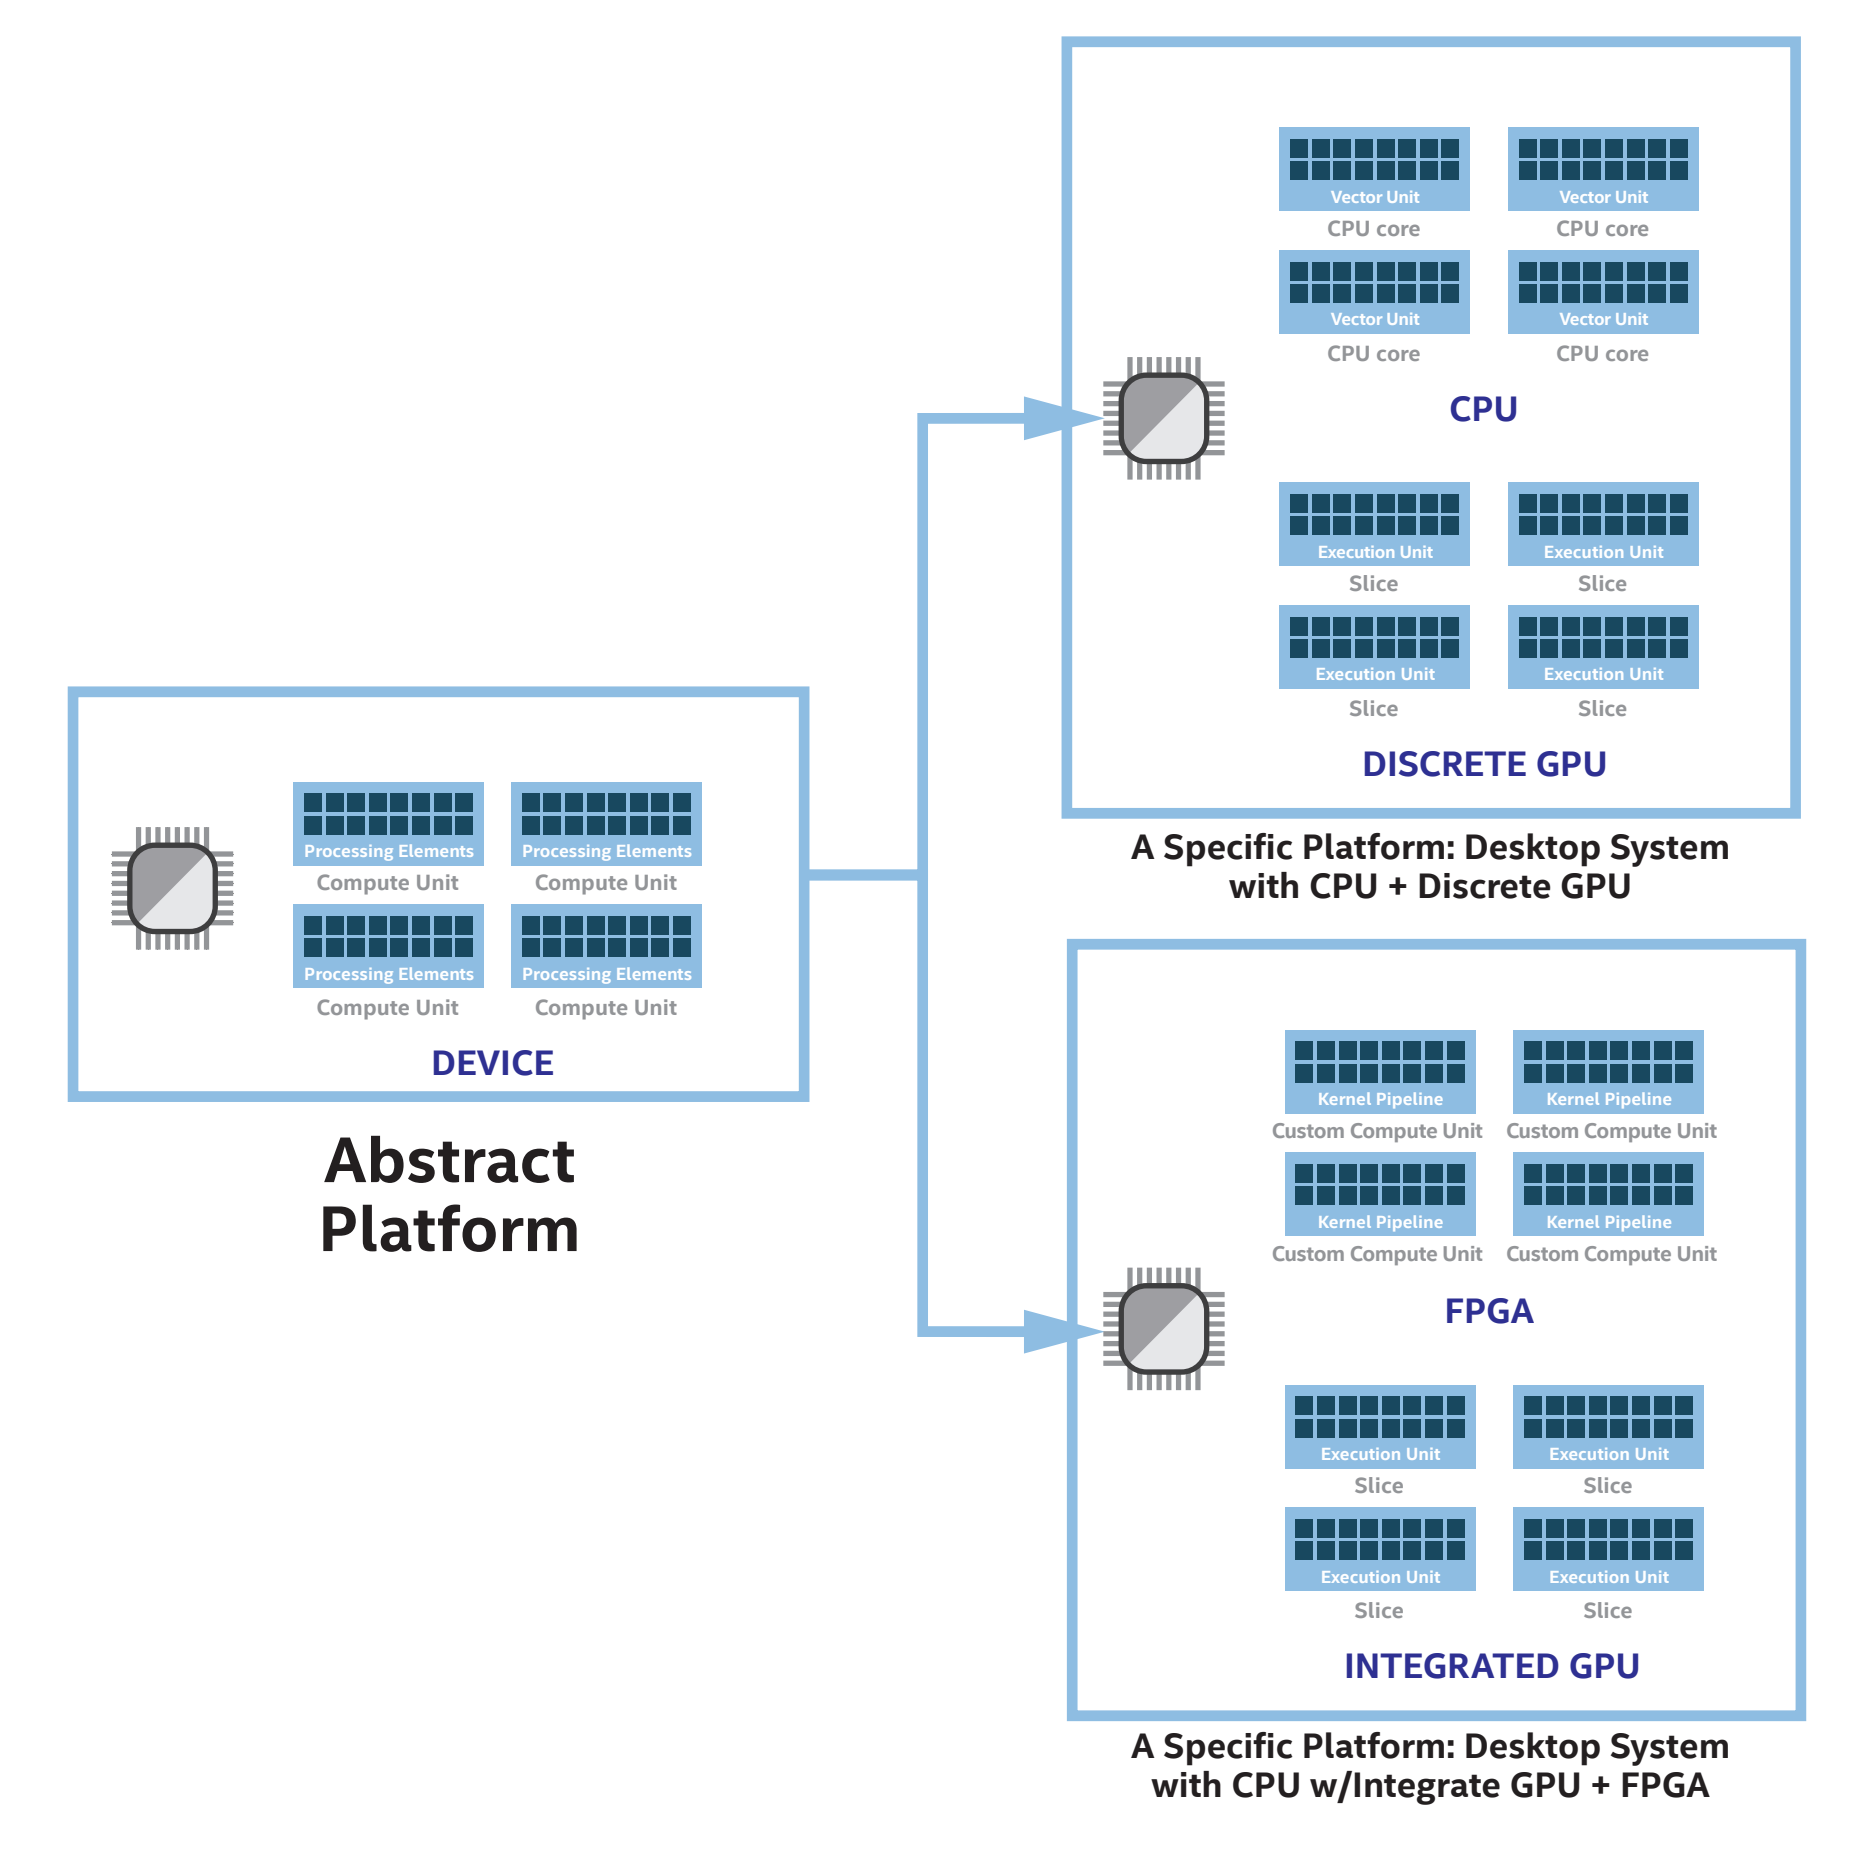
\includegraphics[width=1.\textwidth]{content/chapter-13/images/2}
\end{center}

\hspace*{\fill} \par %插入空行
\textbf{多体系结构二进制文件}

由于我们的目标是使用单一源代码来支持异构机器,因此很自然地希望结果是单个可执行文件。\par

一个多体系结构二进制文件(又名宽二进制文件)是一个单独的二进制文件,已经扩展到包含异构机器所需的所有已编译的和中间代码。多架构二进制文件的概念并不新鲜。例如,一些操作系统支持32位和64位的多架构库和可执行文件。一个多架构二进制文件的作用就像我们常用的任何a.out或A.exe一样,但它包含异构机器所需的一切。这有助于自动的为特定设备选择正确的代码。正如下面要讨论的,一种可能的设备代码形式是中间格式,它将设备指令的最终创建推迟到运行时。\par

\hspace*{\fill} \par %插入空行
\textbf{编译模型}

SYCL和DPC++的单源特性允许编译操作像普通的C++编译。不需要为设备使用额外的工具,也不需要处理设备和主机代码的绑定,这些都由是编译器自动处理。当然,了解事情的细节很重要,原因有几个。如果希望更有效地针对特定的体系结构,这是非常有用的知识,并且了解是否需要调试编译过程中发生的故障也非常重要。\par

回顾编译模型,以便了解何时需要这些知识。由于编译模型支持同时在主机或多个设备上执行的代码,因此编译器、链接器和其他支持工具发出的命令比我们习惯的C++编译(只针对一种体系结构)要复杂得多。\par

DPC++编译器向我们隐藏了这种异构的复杂性。DPC++编译器可以生成与传统C++编译器类似的可执行代码(提前(AOT)编译,有时称为脱机编译),或者可以生成中间表示,可以在运行时将其即时(JIT)编译为特定的目标。\par

只有在设备目标提前已知(编译程序时)时,编译器才能提前编译。延迟即时编译提供了更多的灵活性,但需要编译器和运行时在程序运行时执行额外的工作。\par

\begin{tcolorbox}[colback=red!5!white,colframe=red!75!black]
DPC++编译可以是“提前编译”或“即时编译”。
\end{tcolorbox}

默认情况下,当为大多数设备编译代码时,设备代码的输出以中间形式存储。在运行时,系统上的设备处理程序将实时地将中间形式编译为在设备上运行的代码,以匹配系统上可用的内容。\par

我们可以要求编译器为特定的设备或设备类进行提前编译。这样做的优点是节省运行时间,但缺点是增加了编译时间和更宽的二进制文件!提前编译的代码不如即时编译的代码可移植性好,因为不能在运行时进行调整。我们可以将两者包含在二进制文件中,以获得两者的优点的叠加。\par

提前编译特定设备还有助于在构建时,对设备进行检查。使用即时编译,程序可能会在运行时编译失败(这可以通过第5章中的机制捕捉到)。第5章详细介绍了如何在运行时捕获这些错误,以避免终止程序。\par

图13-2说明了DPC++从源代码到宽二进制文件(可执行文件)的编译过程。无论选择什么组合,都会组合成一个宽二进制文件。宽二进制文件在应用程序执行时由运行时使用(在主机上执行的就是这个二进制文件!)有时,可能希望在单独的编译中编译特定设备的设备代码。希望这样一个单独编译的结果最终组合到宽二进制文件中。完全编译的耗时很长,这对于FPGA开发非常有用,而且实际上FPGA开发需要避免在运行时系统上安装合成工具。图13-3展示了此类需求所支持的绑定/解绑定的流程。总是可以一次编译所有内容,但是在开发过程中,拆分编译的选项会非常有用。\par

每个SYCL和DPC++编译器都有一个相同目标的编译模型,但是确切的实现细节会有所不同。这里显示的图表是DPC++编译器工具链。\par

特定于DPC++的组件如图13-2所示,作为集成头文件生成器,本书中将不再提及。我们不需要知道它是什么,或者能做什么就可以编程。然而,这里有一些信息需要知道:集成头文件生成器会生成一个头文件,提供关于在转译单元中找到的SYCL内核的信息。这包括SYCL内核类型名称如何映射到符号名称,以及关于内核参数及其在相应Lambda或functor对象中的位置的信息,这些信息是由编译器创建。集成头文件是一种机制,用于通过C++ Lambda/functor对象在主机代码上创建内核,可以将我们从设置参数、按名称解析内核等耗时的任务中解放出来。\par

\hspace*{\fill} \par %插入空行
图13-2 编译过程:提前和即时
\begin{center}
	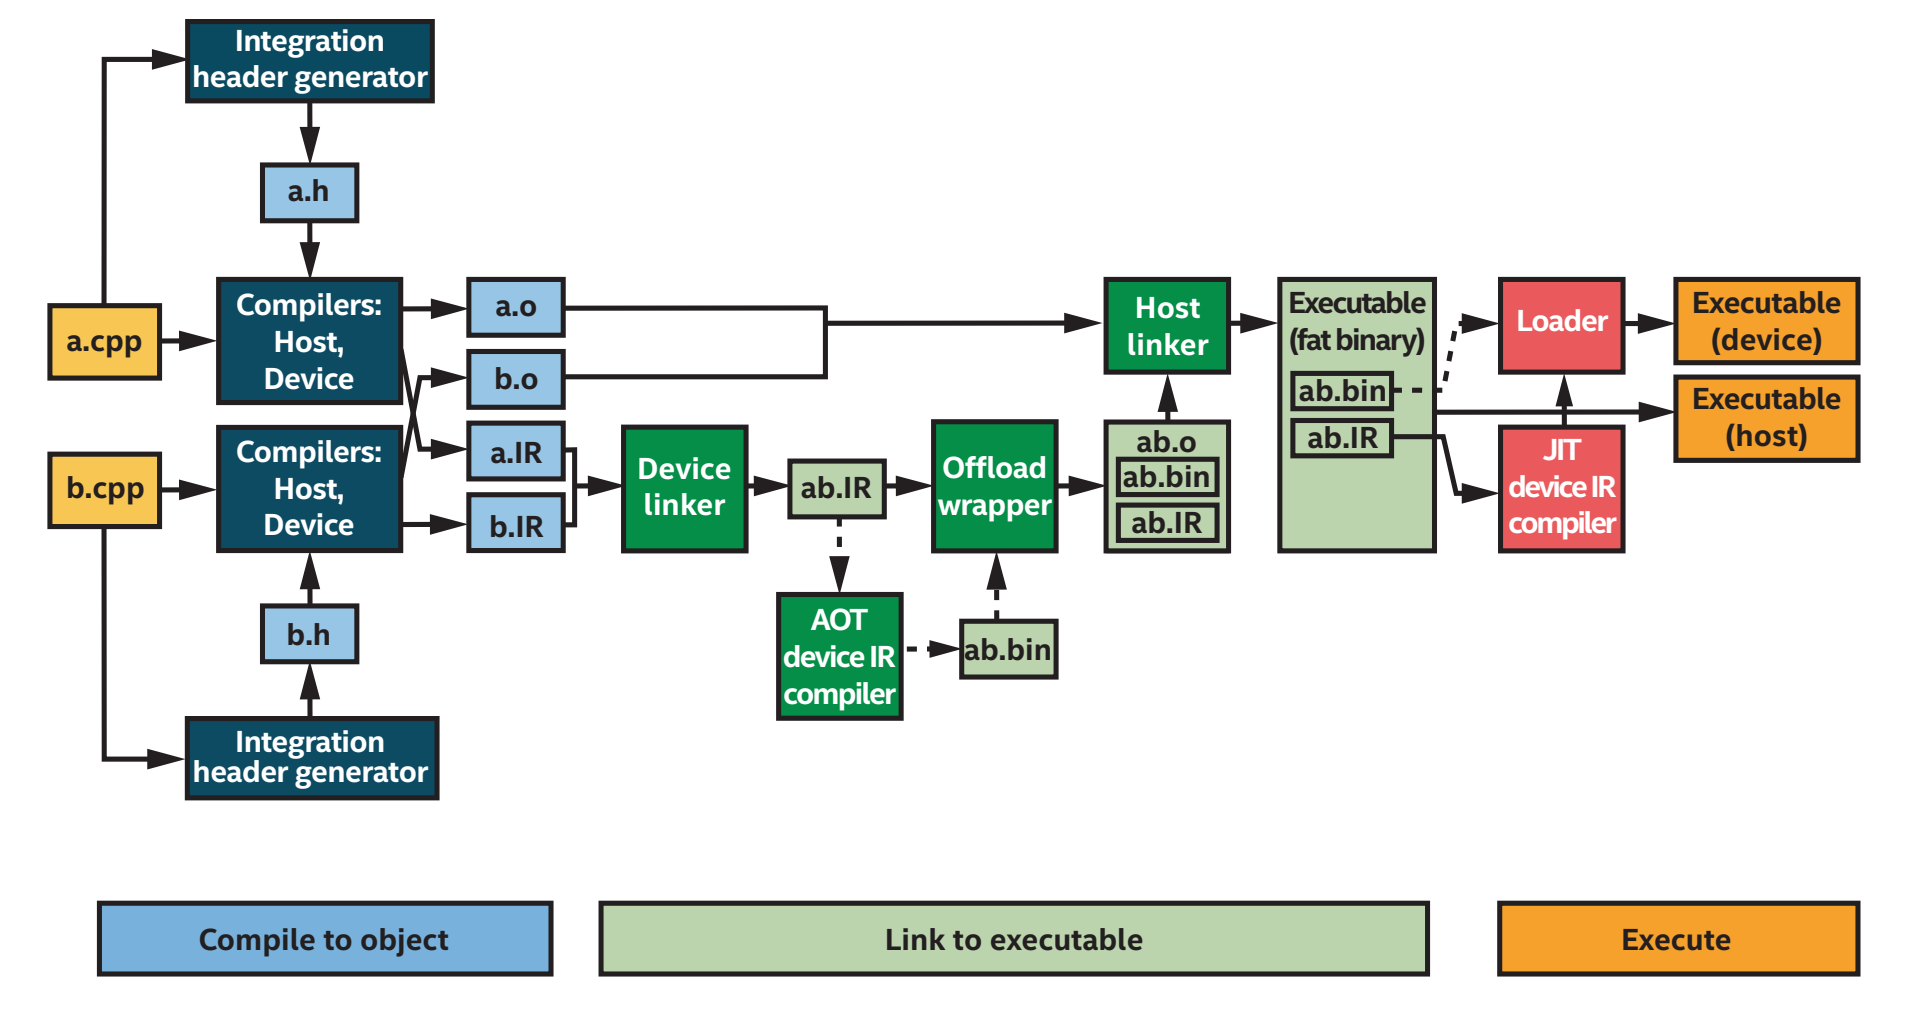
\includegraphics[width=1.\textwidth]{content/chapter-13/images/3}
\end{center}

\hspace*{\fill} \par %插入空行
图13-3 编译过程:组合打包/分解打包
\begin{center}
	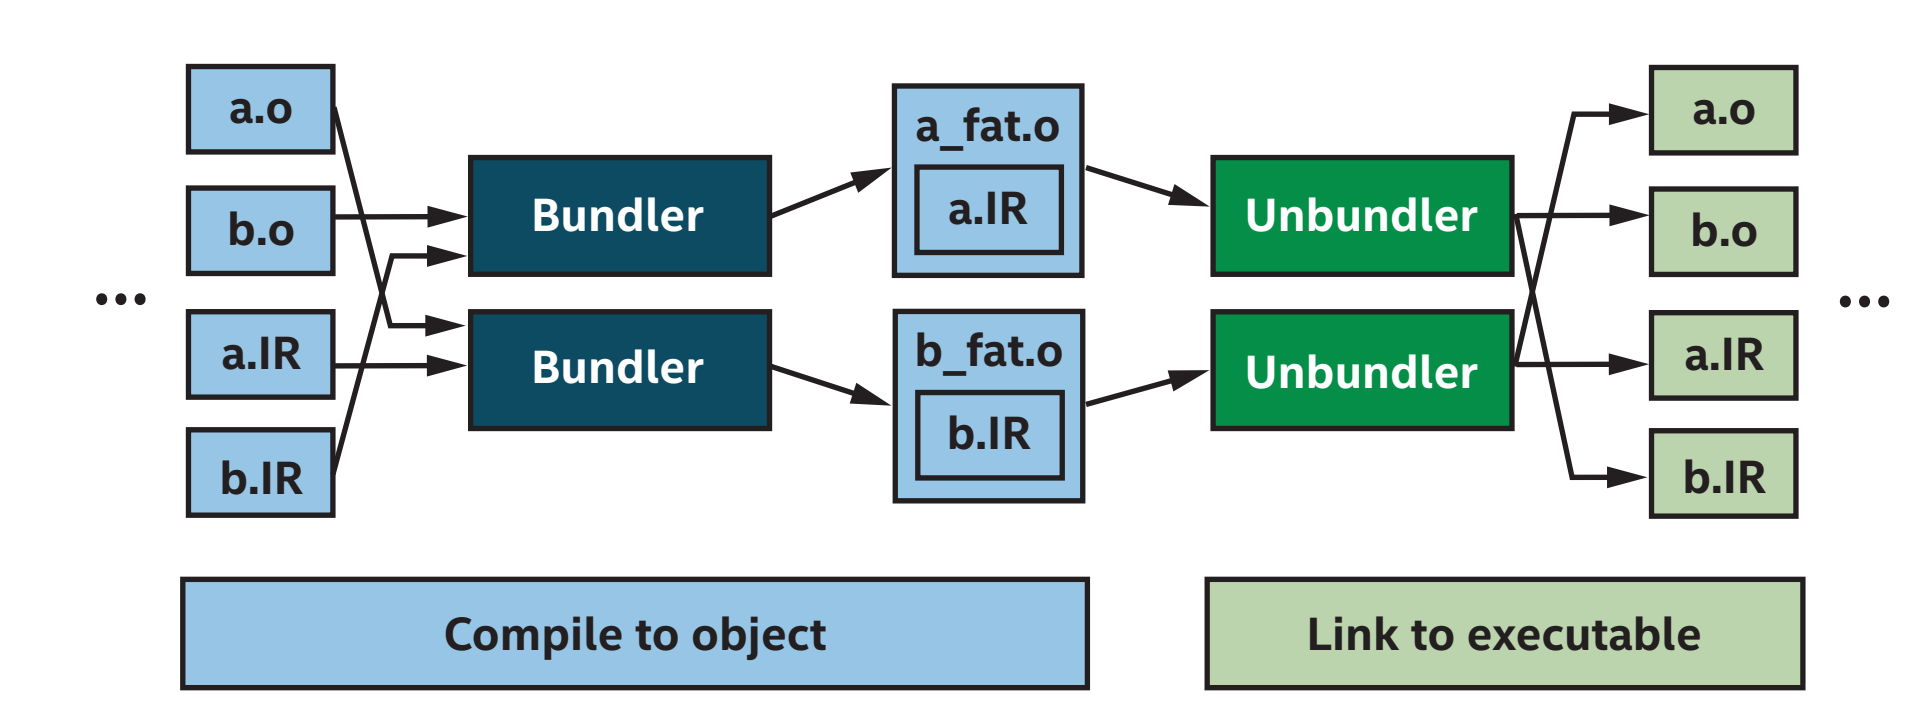
\includegraphics[width=1.\textwidth]{content/chapter-13/images/4}
\end{center}




































